\chapter{背景知识}\label{chapter_background}

本章主要对本文工作的背景知识以及相关工作作相应的介绍。如何保障数值程序的正确性与高效性一直都是软件工程领域的研究热点,研究人员们也提出了许多技术方案。在本章中,我们会简要介绍现阶段较为主流的几种技术方案,包括基于区间算法与仿射算法的静态分析技术,任意精度计算以及用来一些定位数值程序缺陷的测试技术。最后,由于在我们的工作中在进行计算路径提取时也使用到了符号执行的技术,我们对该技术也进行了简要介绍。

\section{浮点数背景知识}

在计算机科学中,浮点数是一种对实数的近似值数值的表示形式。一个浮点数可以以如下的形式表示:
\begin{gather*}
    \pm (1+m) \cdot 2^e
\end{gather*}
其中$m$表示浮点数的有效数字(也被称为尾数),是一个在区间$[ 0 ,\ 1 )$之间的$k$比特的数值,而$e$被称为指数,是一个$l$比特的带符号整数。浮点数可以有不同的精度,例如IEEE754规定的双精度浮点数与单精度浮点数便有着不同的精度,其能够表示的浮点数的范围也不同。双精度浮点数由一个1比特的符号位,53比特的有效数字位以及11比特的指数位组成,而单精度浮点数由一个1比特的符号位,23比特的有效数字位以及8比特的指数位构成。由于浮点数以这样有效数字乘以某个基数的指数的形式表示,同时指数的范围可以很大,所以浮点数能够表示的数值的范围也可以很大,非常大非常小的数均能够由浮点数来表示。

由于浮点数无法准确的表示所有的实数,所以浮点数计算操作的计算结果不一定能够使用浮点数精确的表示,这时浮点数便引入了一种舍入操作,该操作可以将一个实数舍入成为与之非常接近的一个浮点数。舍入操作可以理解为一个函数,其输入是一个实数,输出是一个浮点数。我们使用$\mathsf{F}(r)$表示实数$r$被舍入后得到的浮点数,$\mathsf{R}(f)$表示有浮点数$f$所表示的实数,则浮点数的舍入操作必须能够保证$\mathsf{F(R}(x)) = x $并且$\mathsf{R(F}(x))$是最为接近实数$x$的两个浮点数之一。

\subsection{浮点数误差}

由于浮点数只能够精确的表示能够以$\pm(1+m) \cdot 2^e$形式表示的实数,因此对应那些无法使用浮点数精确表示的实数,舍入操作F必定会引入一定的误差,这样的误差我们称之为舍入误差。对于那些大小适中的浮点数(其以2为底的指数范围在$-2^{l-1}+2$到$2^{l-1}-1$之间的数),其舍入误差主要来自于其有限的有效数字位数。因此舍入误差的大小大概为该实数本身的$2^{-k}$倍左右。例如对于一个大小为$2^{50}$的双精度浮点数,其舍入误差大约为$2^{50} \cdot 2^{-53} = 0.125$左右。我们使用$\mathsf{F}(x) = x + x\epsilon$来表示该转换过程,其中$\epsilon$为实数转换为浮点数过程中的相对误差,对于不同的实数$x$以及在不同的舍入模式下,其相对误差$\epsilon$大小有所不同,但是其绝对值的大小是绝对不会超过$2^{-k}$的。

浮点数的一些基础的计算操作(例如浮点数的加减法)的计算结果能够保证被正确的舍入。举例而言,例如浮点数加法操作$x+y$,其计算结果能够保证是$x$与$y$所表示的实数的加法操作所得到的精确结果被正确舍入后的值:$\mathsf{F}(\mathsf{R}(x)+\mathsf{R}(y))$。也就是说,浮点数加法$x+y$得到的结果其值可以以$x+y+(x+y)\epsilon$这样的形式来表示。

对于其他的浮点数操作,比如说指数函数、三角函数等,其计算过程不能够由计算机硬件直接来完成,必须以函数库的形式来提供。相关的研究工作[]表明,这些复杂的浮点数函数无法达到浮点数加减法这样的精度,对于一般的浮点数函数$f(x_1, x_2, \ldots)$的实现,能够保证其计算结果在与其真实值$\mathsf{F}(f(\mathsf{R}(x_1), \mathsf{R}(x_2) \cdots))$最接近的$2\mu$个浮点数之中。例如$\exp(x)$这个函数,对于一个浮点数输入$x$,其计算结果为$e^x+\mu e^x \epsilon$,通常情况下这里的$\mu$都小于8,也就是说能够保证其计算结果的有效数字中,除了最后两到三位之外,剩余的位置是能够保证正确的。

尽管浮点数的基础的操作是能够达到相当高的精度,然而将这些基础操作结合起来形成的一连串的计算过程仍然有可能是不准确的。举例而言,对于$(x+1)-x = 1$这样一个计算过程,其中第一个加法操作引入的误差为$\epsilon_1$,其得到的计算结果为$x+1+(x+1)\epsilon_1$,紧接着的减法操作引入的误差为$\epsilon_2$,最终得到的计算结果为:
\begin{gather*}
    1+(x+1)\epsilon_1+\epsilon_2+(x+1)\epsilon_1\epsilon_2
\end{gather*}
$\epsilon_2$相对于最终的计算结果1来说非常小,然而对于$(x+1)\epsilon_1$来说,当$x$的值非常大时,该误差有可能是非常大的,甚至对于$(x+1)\epsilon_1\epsilon_2$来说,只要$x$足够大,其也有可能会对最终的计算结果产生影响。因此即便整个计算过程中每一步都是精确的,其最终的计算结果有可能是偏差非常大的。这样的非常相近的很大的两个数进行减法操作在我们现实生活中的软件系统中也是非常常见的,然而这样的操作往往会引起非常大的舍入误差。对于上述的计算过程,在$-1<x<1$时,其计算结果是比较准确的,然而随着$x$的增大,其误差也会随着增大。对于一些更加复杂的计算过程来说,不同输入下的误差大小会有较大的差别,因此如何处理同一个计算过程在不同输入下的误差是我们的工作需要解决的主要问题之一,在本文的工作中,我们对程序的输入域进行了划分以处理不同的误差情况,详情可见第X.X小节。

\section{任意精度计算}

大多数的浮点运算的数值程序使用的是双精度浮点数类型,然而在某些特殊的场景下,双精度浮点类型并不能够满足精度的要求,我们需要使用扩展双精度类型,四精度类型或者更高的精度。在发表于2001年Astronomical Journal的一篇文章中,Toshio Fukushima写道:“在计算机日益强大的今天,源于数值积分的误差仍然是我们研究一些复杂的动态系统,例如用以研究宇宙系统长期运行的稳定性的模拟太阳系和一些地外行星的系统的主要障碍。”他还通过一个实例指出,对于模拟太阳系的系统,双精度浮点数的由于舍入误差积累而导致的误差最终可以达到1弧度之多。此外,对于运行于一些安全攸关或是生命攸关的系统中的浮点程序进行静态分析(例如直升机或者核反应堆中的电子控制系统),也必须使用到任意精度计算。

下面我们举一个实例说明普通的双精度甚至是扩展双精度浮点精度程序有时无法满足我们队精度的要求。假设我们需要计算以下计算式的10位有效数字:
\begin{align*}
    f = 173746a + 94228b - 78487c
\end{align*}
其中:
\begin{align*} 
    a = \sin(10^{22}),\ b = \log(17.1),\ c = \exp(0.42)
\end{align*}
在这个简单的例子中,所有的输入都是精确的,不存在误差,具有无限精度。对应的C代码如图\ref{lst:arbiexcode}所示,我们在64位的Fedora10操作系统上,使用GCC4.3.2编译器,使用2.9版本的GNC C库,运行该代码,我们可以得到其计算结果为$d = 2.9103830456733704\text{E}-11$,这个结果很显然是完全错误的,其准确的结果为$d = −1.341818958\text{E}−12$。我们将该计算过程使用的双精度类型修改为扩展的双精度类型(64位有效数字),同时我们也将使用到的函数修改为对应扩展双精度的版本,将sin($10^{22}$)改为sinl($10^{22}$),将log修改为logl,将exp改为expl,我们得到的结果为$d=-1.3145040611561853E−12$,这个结果和之前的答案一样都是错误的。很显然,我们在计算时使用的精度不够。

\begin{figure}[thbp]
    \begin{lstlisting}[%
      xleftmargin=5em,numberblanklines=true,boxpos=b,%,extendedchars=\true, %inputencoding=utf8%/latin1
      morekeywords={REAL,IComplex}%keywords={main}
    ]
    #include <stdio.h>
    #include <math.h>

    int main(void) {
        double a = sin (1e22), b = log (17.1);
        double c = exp (0.42); double d = 173746*a +
        94228*b - 78487*c; printf ("d=%.16e\n", d); 
        return 0;
    }

    \end{lstlisting}
    %\vspace*{-4mm}
    \caption{计算$f = 173746a + 94228b - 78487c$的C代码}
    \label{lst:arbiexcode}
    %\vspace*{-4mm}
\end{figure}

我们可以简单分析一下上述程序出错的原因,首先常数如$10^{22},17.1$或者$0.42$可能无法以二进制精确的表示。对于常数$10^{22}$,编译器能够将其转换为正确的二进制数,并符合IEEE754标准,它能够在双精度浮点数下精确的表示,因此不存在这个问题。然而对于$17.1$以及$0.42$来说,他们都不能以二进精确的表示,与$17.1$最为接近的双精度浮点数为$2406611050876109\cdot2^{−47}$,这与真实值相差$1.4\cdot10^{-15}$,$0.42$也类似。

其次,IEEE754标准并没有规定数学函数如sin,log,exp要进行正确的舍入,就连精度都没有要求,这导致计算结果完全取决于所使用的平台。我们计算的$a,b,c$可能会使用正确的舍入方法得到的结果相差一些最小精度单位。

最后,在整个计算过程中出现了相近数相减的操作,假设我们从左往右进行计算,$173746a+94228b$和$78487c$分别舍入为:
\begin{align*}
x & =1026103735669971·2^{-33}≈119454.19661583972629 \\
y & =4104414942679883·2^{-35}≈119454.19661583969719
\end{align*}
根据Sterbenz定理[],计算$x−y$不存在舍入误差。但最终结果的精确度明显地由计算$x$和$y$的舍入误差决定, 约为$2^{-36}≈1.5·10^{-11} $.由于要求的真值与此误差大小相近, 这样就导致了我们的最终计算结果$d$完全错误。

任意精度计算是指用户能够选择每个运算的计算精度,任意精度计算也被称作多精度计算,因任意精度计算的计算过程中,其数值的有效数字位是动态的存储在多个机器字节中的,当计算精度要求较高时,所分配的机器字节也随之增多,以保证计算精度。当前许多语言都有支持任意精度计算的数值计算库,同时绝大多数计算代数系统也支持任意精度计算,例如Mathematica、Maple和sage等。下面我们简单介绍两个任意精度的数值计算库,一个是GNU MPFR,另一个是iRRAM。

\subsection{GNU MPFR}

GNU MPFR是一个用户任意精度浮点运算的C语言库,其在计算过程中能够保证正确的舍入操作,所以在不同的平台下其计算结果也能够保证完全一致。MPFR库的主要特点有:

\begin{enumerate}
\item 支持一些特殊的数值,如带符号的0(-0),正负无穷,NaN等
\item 每一个数值都带有其自己精度信息,每一个浮点运算的结果都会根据该精度被正确的进行舍入
\item 支持所有常用的数学函数,其实现了C99标准中所有的数学函数以及另外一些常用的数学函数,例如对数函数、指数函数等
\end{enumerate}

我们之前的程序可以使用MPFR改写为如图\ref{lst:arbiexmpfrcode}的代码:

\begin{figure}[thbp]
    \begin{lstlisting}[%
      xleftmargin=7em,numberblanklines=true,boxpos=b,%,extendedchars=\true, %inputencoding=utf8%/latin1
      morekeywords={REAL,IComplex}%keywords={main}
    ]
    #include <stdio.h>
    #include <stdlib.h>
    #include "mpfr.h"
    int main (int argc, char *argv[])
    {
       mp_prec_t p = atoi (argv[1]);
       mpfr_t a, b, c, d;
       mpfr_inits2 (p, a, b, c, d,(mpfr_ptr) 0);
       mpfr_set_str (a, "1e22",10, GMP_RNDN);
       mpfr_sin (a, a, GMP_RNDN);
       mpfr_mul_ui (a, a, 173746, GMP_RNDN);
       mpfr_set_str (b, "17.1",10, GMP_RNDN);
       mpfr_log (b, b, GMP_RNDN);
       mpfr_mul_ui (b, b, 94228, GMP_RNDN);
       mpfr_set_str (c, "0.42",10, GMP_RNDN);
       mpfr_exp (c, c, GMP_RNDN);
       mpfr_mul_si (c, c, -78487, GMP_RNDN);
       mpfr_add (d, a, b, GMP_RNDN);
       mpfr_add (d, d, c, GMP_RNDN);
       mpfr_printf ("d =%1.16Ren", d);
       mpfr_clears (a, b, c, d, NULL);
       return 0;
    }
    \end{lstlisting}
    %\vspace*{-4mm}
    \caption{计算$f = 173746a + 94228b - 78487c$的C代码}
    \label{lst:arbiexmpfrcode}
    %\vspace*{-4mm}
\end{figure}

此程序的输入p为计算精度。\\
若我们取p=53,其运行结果为d = +2.9103830456733704e-11,这与我们使用双精度浮点数所得的结果完全一致;\\
若我们取p=64,其运行结果为 d = -1.3145040611561853e-12,这与我们使用扩展双精度结果一致;\\
若我们取p=113,对应于IEEE754标准的四精度类型,其运行结果为 d = -1.3418189578296195e-12,此结果与正确结果完全一致;

\subsection{iRRAM}

iRRAM是一个非常高效的C++任意精度数值计算库,其基于图灵机模拟了一个随机存取机来完成对数值计算操作。iRRAM在进行数值计算时会不断的进行迭代,并在每次迭代时都增加所使用的精度。在本文所介绍的工作中,所有涉及到的任意精度程序均是使用iRRAM任意精度数值计算库实现的。

我们在使用iRRAM时,可以使用一种特殊的数值类型REAL,我们可以像对待实数一样对待该类型的变量,使用REAL类型的变量进行计算操作是绝对不存在任何误差的。我们也可以使用REAL类型定义自定义数据类型,例如矩阵,复数等等,还可以使用REAL类型实现各种各样的数学函数。iRRAM库已经帮助我们实现了一系列常用的数学函数,包括了三角函数、反三角函数、对数指数函数、幂函数等等。

我们在使用iRRAM时还有一些注意事项,首先,用户无法使用普通的IO操作,必须使用iRRAM自己实现的IO库,否则可能会导致错误的输入输出。其次,数值计算程序中无法使用全局的REAL类型的变量,用户必须尽可能少地使用malloc函数来动态分配内存,可以使用alloca来动态分配内存。由于iRRAM的特殊语义,在使用第三方库时也必须倍加小心。

下面以一个具体的iRRAM程序来简要介绍一下iRRAM程序的特点和使用方法,如图\ref{lst:arbiexmpfrcode}所示的iRRAM程序。

\begin{figure}[thbp]
    \begin{lstlisting}[%
      xleftmargin=3em,numberblanklines=true,boxpos=b,%,extendedchars=\true, %inputencoding=utf8%/latin1
      morekeywords={REAL,IComplex}%keywords={main}
    ]
    #include "iRRAM.h"
    REAL maxapprox (long k, const REAL& x, const REAL& y)
    { if ( positive(x-y,k) ) return x; else return y; };
    REAL max (const REAL& x, const REAL& y)
    { return limit(maxapprox,x,y); };
    void compute()
    {   REAL x1 = 3.14159, x2 = "3.14159", x3 = pi();
        rwrite(x1,63); rprintf("\n"); 
        rwrite(x2,63); rprintf("\n"); 
        rwrite(max(x3,x2),63); rprintf("\n"); }
    int main (int argc,char **argv)
    { iRRAM_initialize(argc,argv); iRRAM_exec(compute); }
    \end{lstlisting}
    \begin{align*}
        +.3141589999999999882618340052431449294090270996093750000\text{E}+0001 \\
        +.3141590000000000000000000000000000000000000000000000000\text{E}+0001 \\
        +.3141592653589793238462643383279502884197169399375105821\text{E}+0001
    \end{align*}

    %\vspace*{-4mm}
    \caption{iRRAM示例程序代码}
    \label{lst:irramexcode}
    %\vspace*{-4mm}
\end{figure}



\section{静态分析方法}
在数值计算的研究领域,一些静态的程序分析技术被提出以研究程序可能产生的误差范围以及定位产生误差的计算操作,这些静态分析技术主要基于区间算术理论以及仿射算术理论。在本小节中,我们会主要介绍区间算术和放射算术的一些基本概念以及运算操作,阐述两者的各自的特点以及优缺点。另外,我们会简要介绍基于这两种技术的数值计算程序的一些相关工作。

\subsection{区间算法}

区间算术(Interval Arithmetic)也称作区间分析,其定义了在区间上的一系列运算操作,主要特点是可以处理不确定数据,分析计算机中浮点操作的截断误差与舍入误差,高效而可靠地估计函数在自变量区域的取值范围,从而被广泛应用于自然科学的各个研究领域,包括光线追踪,实体建模,全局优化等等。近些年来,区间算术也被应用于系统的可行域或者可靠性分析之中。

区间算数使用闭区间$[a, b]$代表该区间内所有的实数:

\begin{equation*}
    [a, b] = \{x \in \mathbb{R} : a \leq x \leq b \}
\end{equation*}

区间算法定义了一系列包括加减乘除的区间之间的计算操作,若以$\odot$代表这些计算操作,则我们有:

\begin{equation*}
    X \odot Y = \{ a \odot b : a \in X , b \in Y \}
\end{equation*}

对于区间$X = [\underline{X},\ \overline{X}],\ Y = [\underline{Y},\  \overline{Y}]$,其加减乘数四则运算,我们有如下计算公式:
\begin{align*}
    X + Y & = [\underline{X} + \underline{Y},\ \overline{X} + \overline{Y}] \\
    X - Y & = [\underline{X} - \overline{Y},\ \overline{X} - \underline{Y}] \\
    X \times Y & = [\min S ,\ \max S],\ S = \{\underline{XY},\ \underline{X}\overline{Y},\ \overline{X}\underline{Y},\ \overline{XY}\} \\
    X \div Y & = [\min T,\ \max T],\ T = \{\underline{X}/\underline{Y},\ \underline{X}/\overline{Y},\ \overline{X}/\underline{Y},\ \overline{X}/\overline{Y} \} \\
\end{align*}
区间算术存在一个很大的问题在于其进行区间分析得到的结果区间往往比精确的结果区间大很多倍。举一个很简单的例子,对于计算式$f(x) = x - x$,给定$x \in X = [2,\ 5]$,我们使用区间的减法操作得到的结果是$[-3,\ 3]$,而不是$[0,\ 0]$。这主要是由于区间算术没有“记忆功能”,其无法分辨两个区间实际上指代的是同一个区间。
更加一般的情况,我们考虑一个计算过程$z \leftarrow f(x, y)$,如果其计算的输入$x,\  y$具有相关性,则其计算得到的结果$\overline{z} \leftarrow \overline{f}(\overline{x},\ \overline{y})$将比精确的结果区间$z$大上许多倍。我们可以定义一个高估因子$\sigma$为区间分析得到的结果区间的宽度除以其精确结果区间的宽度,$\sigma$越大则代表区间分析的结果越不准确。研究工作表明,高估因子$\sigma$的大小主要取决于$x$与$y$的相关系数的正负和大小以及$f$的导数,与$x,\ y$原始的区间大小无关。举例而言,对于计算式$f(x)=x(10-x)$,对于$x \in [3,\ 5]$,其区间分析结果为$[15,\ 35]$,其区间宽度为是精确的结果区间$[21,\ 25]$的5倍,如果我们将原输入区间缩小为$[3.9,\ 4.1]$,区间分析的结果是$[23.01,\ 25.01]$,其宽度依旧为精确结果区间$[23.79,\ 24.19]$宽度的5倍。
由于存在这样的问题,导致区间分析技术难以被更为广泛的应用。尤其在一些链式计算中,上一步的计算结果需要作为下一步的计算输入这样的情况,每一个独立的计算步骤的高估因子都会以相乘,导致最后的整个区间分析的结果区间异常的大,这样的结果是无法使用的。

\subsection{仿射算法}

仿射算法(Affine Arithmetic)是新近出现的处理不确定性问题的方法,其不仅记录了每个输入的区间,同时还记录了每个输入之间的相关性信息。在仿射算术中,一个不确定量(区间)$x$可用一个仿射形式表示,它是一些噪声元的线性组合:
\begin{align*}
    \hat{x}  = x_0\varepsilon_0 + x_1\varepsilon_1 + ... + x_n\varepsilon_n = x_0 + \sum_{i=1}^{m}x_i\varepsilon_i
\end{align*}
上述定义中每个$\varepsilon_i$都代表了$x$的一个不确定性来源,其范围在$[-1,\ 1]$之间,这些不确定性可能是“内部”的(例如由于舍入误差或近似计算引入的不确定性),亦有可能是“外部”的(例如输入本身存在的误差),而每一个系数$x_i$都代表了每个不确定性来源的系数大小。

给定两个仿射形式$\hat{x}  = x_0\varepsilon_0 + x_1\varepsilon_1 + ... + x_n\varepsilon_n$和$\hat{y}  = y_0\varepsilon_0 + y_1\varepsilon_1 + ... + y_n\varepsilon_n$,假设$a$是常数,对于线性运算,可以定义:
\begin{gather*}
    \hat{x} \pm \hat{y} = (x_0 \pm y_0) + (x_1 \pm y_1)\varepsilon_1 + ... + (x_n \pm y_n)\varepsilon_n \\
    \alpha \pm \hat{x} = (\alpha \pm x_0) + x_1\varepsilon_1 + ... + x_n\varepsilon_n \\
    \alpha \hat{x} = (\alpha x_0)\varepsilon + (\alpha_1 x_1)\varepsilon_1 + ... + (\alpha x_n)\varepsilon_n
\end{gather*}
可见,对于线性运算,仿射运算不引入新的误差。

仿射形式与区间形式之间是可以通过一定的方法相互转换的,每个以仿射形式表示的变量$\hat{x}  = x_0\varepsilon_0 + x_1\varepsilon_1 + ... + x_n\varepsilon_n$都可以使用一个区间变量来表示 $x \in X = [x_0 - r,\ x_0 + r]$,其中$r = \sum_{i=1}^{n} |x_i| $,由于每个$\varepsilon_i$都属于$[-1,\ +1]$,这是包含所有可能的x的值的最小区间。

与此对应的,每个以区间形式$ x \in X = [a,\ b]$表示的变量$x$,都能够以仿射形式$\hat{x} = x_0 + x_k\varepsilon_k$表示, 其中$x_0$为区间$X$的中点$(a+b)/2$,$x_k$是区间$X$的半径$(b-a)/2$,$\varepsilon_k$是一个新的噪声源。

仿射算术最主要的特点是同一个噪声源能够出现在不同的变量(可以是输入,输出亦或是中间变量)中,这样便提供了变量之间的相关性信息。举例而言,假设我们有如下仿射形式的$\hat{x}$与$\hat{y}$:
\begin{align*}
    \hat{x} = 20 - 4\varepsilon_1 \qquad \quad + 2\varepsilon_3 + 3\varepsilon_4 \\
    \hat{y} = 10 - 2\varepsilon_1 + 1\varepsilon_2 \qquad \quad - 1\varepsilon_4
\end{align*}

我们可以知道$x$属于区间$[11,\ 29]$,$y$属于区间$[6,\ 14]$,因此,若使用区间分析的技术,我们可以直接得到点$(x,\ y)$所属区域为图\ref{fig:interval_affine_diff}中的浅灰色区域,是一个矩形。然而若使用仿射算术的方法去分析该问题,由于$x$与$y$共享两个噪声源$\varepsilon_1$与$\varepsilon_4$,我们遍历所有可能的$\varepsilon_1,\ \varepsilon_2,\ \varepsilon_3,\ \varepsilon_4$的取值,可以得到$(x,\ y)$所属区间实际上为图\ref{fig:interval_affine_diff}中的深灰色区域。由此可见,仿射算术由于利用到了变量之间的相关性信息,在处理线性运算时,可以得到比区间算数更为准确的结果。

\begin{figure*}[thbp]
    \centering
    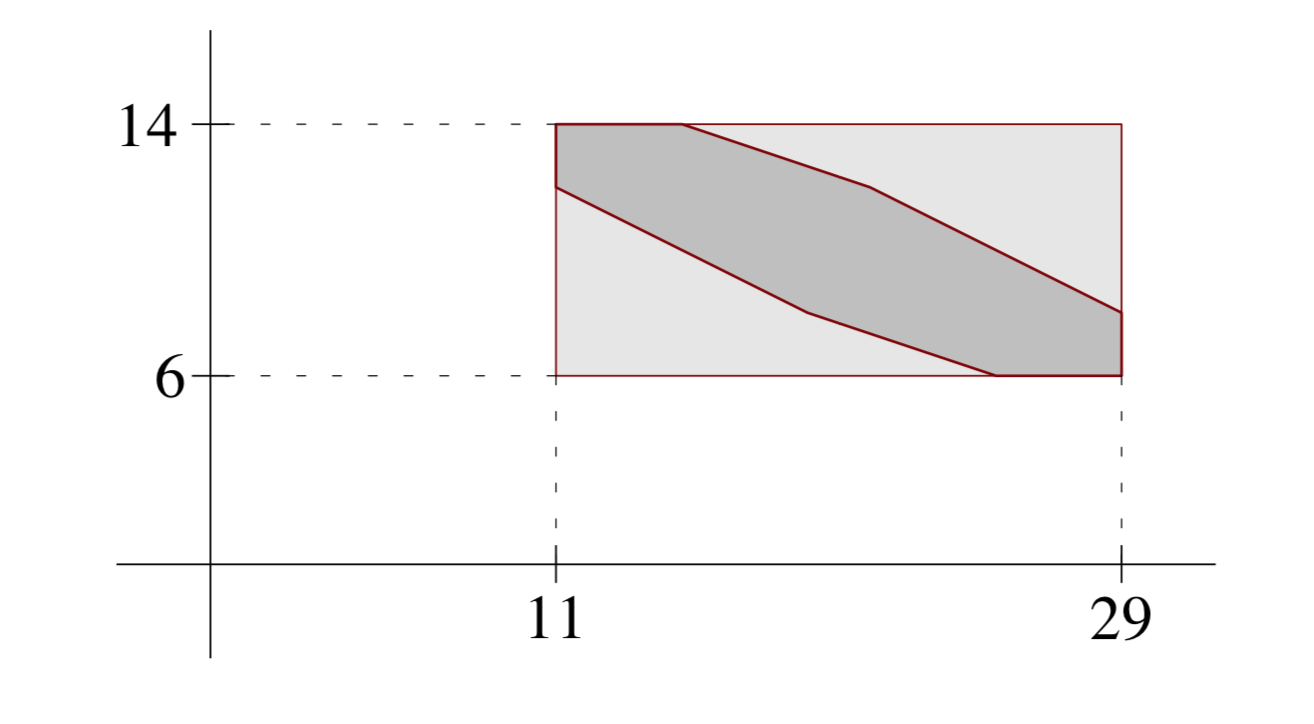
\includegraphics[width=88mm]{fig/IntervalAffineDiff.png}
    \caption{区间算法与仿射算法分析结果对比} \label{fig:interval_affine_diff}
\end{figure*}

然而不幸的是,仿射算术并不是在所有情况下都能够比区间算术得到更加准确的结果,如对于非线性运算,特别是由乘除指数开方等构成的复合运算,误差的减小不是绝对的。如区间变量$x \in X = [1,\ 2]$,在计算$f(x) = 1/x$时,利用区间算术的运算规则可以得到其结果为$[1/2 ,\ 1]$,然而使用仿射算术,我们首先需要将$x$改写成仿射形式$\hat{x} = 1.5 + 0.5\varepsilon_1$,然后再使用倒数运算的仿射公式,求得其结果区间为$[0.4142,\ 1]$。

由此可见,由于仿射算法在处理非线性运算时会引入新的误差,所得的界限不一定比区间算法的运算结果紧凑.故在计算函数界限时,需要针对不同函数选取不同算法以期尽快获得尽量紧凑的函数界限.

基于区间算法以及仿射算法,许多静态分析方法被提出以研究数值计算程序中浮点数计算的误差积累情况。Putot提出了一种针对C代码静态分析技术,其研究了在C程序中每一步计算过程中浮点计算的误差积累情况,通过区间分析的方法,将计算过程中每一步的误差以一个区间的形式表示,对程序进行抽象释义,能够发现程序中引起严重的精度损失的计算操作,也能够验证程序最终的执行结果在一定的误差范围之内。[]后续Goubault和Putot使用仿射算法改进了这一静态分析方法,使得该分析方法能够应对一些更加复杂的数值程序,例如解非线性方程的牛顿法、共轭梯度法等的数值程序,同时也极大的提升了分析结果的准确性。[]


\section{符号执行技术}

\subsection{符号执行具体原理}

符号执行是一种广泛用于程序分析、软件安全和软件测试的技术,该技术 在20世纪70年代就被提出,从提出至今已经取得了长足的发展。符号执行可以帮助人们完成高覆盖率的测试用例生成以及发现并定位一些复杂软件系统中非常隐蔽的缺陷。在软件测试领域,符号执行的主要目标是能够高效的探索尽可能多的不同的程序执行路径。对于每一条执行路径,符号执行可以通过约束求解的方式生成触发该执行路径的具体输入,另外还可以检测该执行路径上是否有程序缺陷,包括内存溢出、未捕获的异常等等。从软件测试的角度来看,符号执行可以帮助我们生成高覆盖率的测试用例,从缺陷检测的角度来看,符号执行可以提供能够除法特定缺陷的具体输入,以帮助程序员调试代码,修正缺陷。

符号执行的核心思想是使用符号化的变量而非具体的程序输入去执行程序,程序中所有的中间变量都由符号化的输入变量的表达式来表示,程序最终的输出也不是一个具体的数值,而是一个以符号化的输入变量为参数的一个函数。除了将程序中的输入替换为符号化输入以外,对于每一条程序执行路径,符号执行还需要维护该路径对应的符号执行状态$\sigma$以及路径约束$PC$,其中符号执行状态$\sigma$是一张程序变量与其对应的符号化表达式的对应关系表,而路径约束$PC$通常有一组符号化表达式的交集构成,代表了执行该条路径时程序输入所需要满足的条件。符号执行状态$\sigma$以及路径约束在符号执行过程中都会不断地进行更新,在符号执行结束后,我们可以调用底层约束求解器对路径约束进行求解,求解得到的结果作为程序的具体输入值则可以触发该条执行路径。符号执行会尝试遍历程序的所有路径, 而符号执行过程中的所有程序路径可以通过一棵符号执行树进行表示。

通过以上描述,我们可以总结出符号执行不同于具体执行的几个主要特征:
\begin{itemize}
    \item 符号执行使用符号化的输入代替具体值输入,并将程序中所有变量都使用符号化输入构成的表达式进行表示。
    \item 符号执行为每一条执行路径维护了一个执行状态表$\sigma$以及路径约束$PC$,在符号执行结束时调用约束求解器求解约束得到能够触发该执行路径的程序具体输入。
    \item 程序往往具有多条执行路径,而具体输入一次只能触发其中一条执行路径,而符号执行中程序的所有执行路径构成了一个符号执行树,通过对符 号执行树的所有路径进行遍历,即可完成对程序所有执行路径的遍历。
\end{itemize}

为了更加进一步的说明符号执行于具体执行的区别,我们以图\ref{lst:symexeccode}所示的示例程序来介绍具体执行以及符号执行的不同的执行过程。
\begin{figure}[thbp]
    \begin{lstlisting}[%
      xleftmargin=10em,numberblanklines=true,boxpos=b,%,extendedchars=\true, %inputencoding=utf8%/latin1
      morekeywords={sym_input, ERROR}%keywords={main}
    ]
    int triple(int v) {
        return 3*v;
    }

    void sym_example(int x, int y) {
        z = triple(y);
        if (z == x) {
            if (x > y + 5) {
                ERROR;
            }
        }
    }

    int main() {
        x = sym_input();
        y = sym_input();
        sym_example(x, y);
        return 0;
    }
    \end{lstlisting}
    %\vspace*{-4mm}
    \caption{符号执行示例程序代码片段}
    \label{lst:symexeccode}
    %\vspace*{-4mm}
\end{figure}

在具体执行时,我们假设程序的具体输入是$\{x=3,y=1\}$,程序的具体执行过程如下:执行语句6,其会调用函数triple,返回结果是3,因此,变量$z$被赋值为3;然后顺序执行语句7,是一个if语句,此时$z$与$x$的具体值均为3,满足$z==x$,因此进入该分支;执行语句8,依然为if语句,不满足条件$x>y+5$,程序具体执行结束。由此可见,具体执行只执行了函数sym\_example多条执行路径中的一条。

在符号执行时,首先会创建一个执行状态$\sigma$以及路径约束$PC$,在一开始的时候$\sigma$是一个空集,$PC$为$true$。每当遇到一个语句$var = sym_input()$时,符号执行会将一个新的符号与变量之间的对应关系$var \mapsto s$添加到a中去,这里的$s$是一个新的符号化的变量。在这个例子中,程序的第15-16行会使得原本为空的$\sigma$更新为$\sigma = \{x \mapsto x_0, y \mapsto y_0\}$;每当遇到一个赋值语句$v = e$时,符号执行会将执行状态$\sigma$中的$v$的表达式更新为$\sigma(e)$,也就是使用当前执行状态中的对应关系计算$e$得到的结果。在这个例子中,当我们执行完语句6时,程序的执行状态会被更新成为$\sigma = \{x \mapsto x_0, y \mapsto y_0, z \mapsto 3x_0\}$;每当遇到一个条件分支语句 \texttt{if (}$e$\texttt{) S1 else S2}时,$PC$会被更新成为$PC\wedge\sigma(e)$,对应then分支,同时也会产生一条新的执行路径,其路径约束为$PC'=PC\wedge\neg\sigma(e)$,对应了else分支,这里便不同于具体执行,因为具体执行仅仅会执行这两条分支中的一条,而在符号执行过程中,每一条执行路径均会被记录下来。在此例中,当我们执行完语句7后,会产生两条不同的执行路径分别对应$x_0 = 3y_0$以及$x_0 \neq 3y_0$,同样的,在执行完语句8后,在$x=3y_0$的分支亦会产生两个新的执行路径,其对应的路径约束分别为$(x_0 = 2y_0) \wedge (x_0 > y_0 + 5)$与$(x_0 = 2y_0) \wedge (x_0 \leq y_0 + 5)$。当符号执行遇到结束语句后,当前的符号执行实例便终止了,然后对调用底层求解器求解路径约束得到路径对应的程序的具体输入,在这个具体的例子中,我们可以求解得到三条路径对应的不同的具体输入分别为$\{x = 0,y = 1\}$,$\{x = 3,y = 1\}$和$\{x = 30, y = 10\}$。最终的符号执行结果如表\ref{tbl:symexamres}所示,其符号执行树如\ref{fig:symexectree}所示;

\begin{table}
    \centering
    \begin{tabular}{ccc}
      \toprule
      \textbf{程序路径} & \textbf{路径约束} & \textbf{测试用例} \\
      \midrule
      路径1 & $3y_0 = x_0 \wedge x_0 > y_0 + 5$ & $x = 30, y = 10 $ \\
      路径2 & $3y_0 = x_0 \wedge x_0 \leq y_0 + 5 $ & $x = 3, y = 1$ \\
      路径3 & $3y_0 \neq x_0$ & $x = 0, y = 1$ \\
      \bottomrule
    \end{tabular}
    \caption{程序sym\_example基于符号执行生成的测试用例}\label{tbl:symexamres}
\end{table}

\begin{figure*}[hbp]
    \centering
    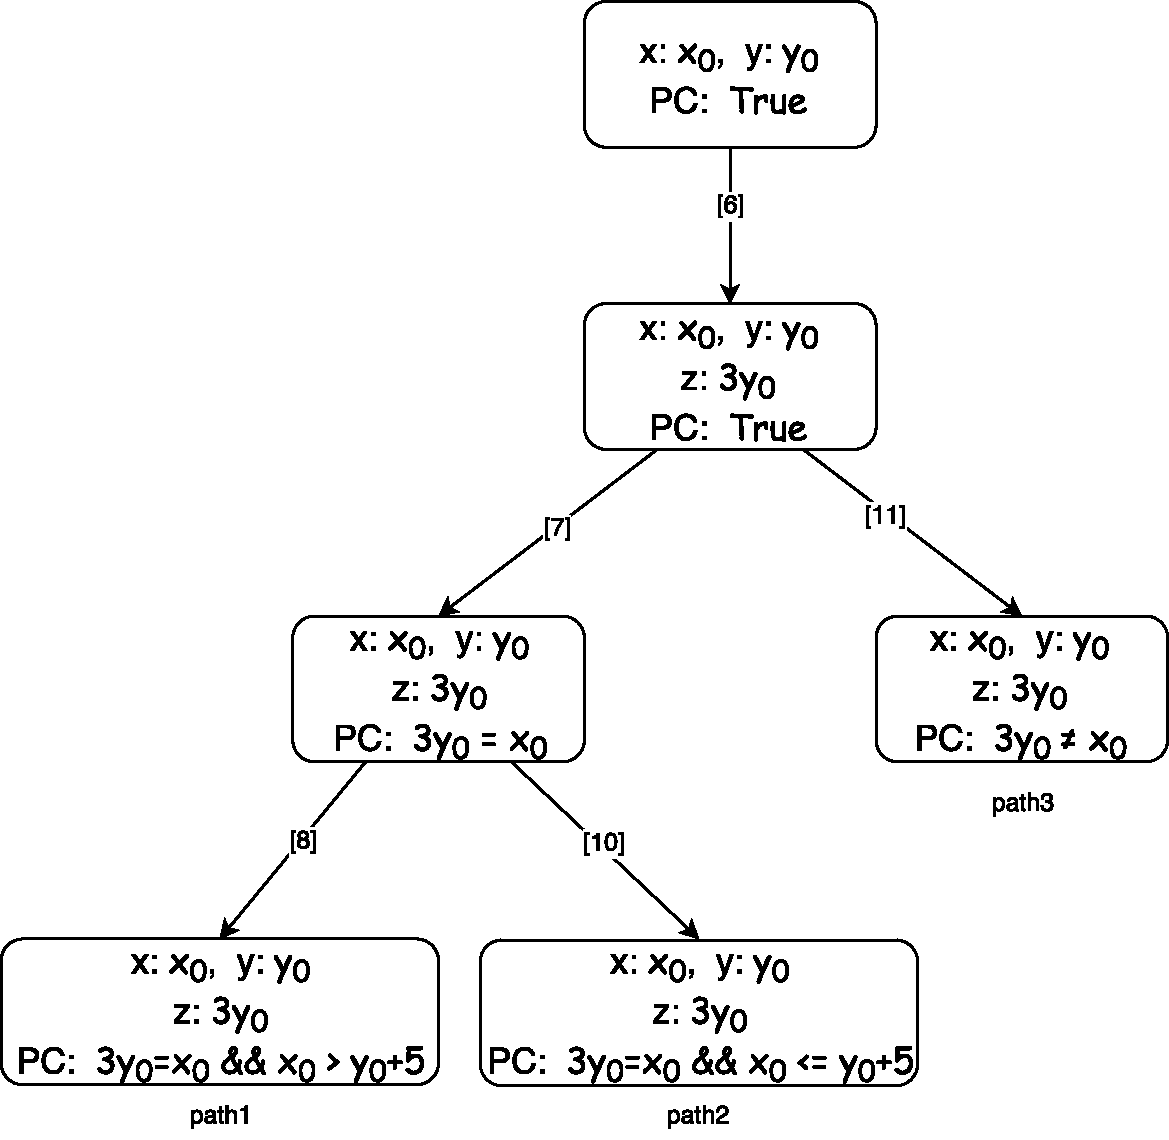
\includegraphics[width=100mm]{fig/SymExecTree.pdf}
    \caption{程序sym\_example符号执行树} \label{fig:symexectree}
 \end{figure*}


在这一小节中,我们简要介绍了符号执行的基本原理以及其余具体执行的主要区别。在本文工作中,我们使用符号执行过程对一个数值计算程序的整体的计算过程进行了提取,提取的结果是程序的输出关于程序输入的一个计算式的形式,从上述对符号执行的描述我们可以知道,该计算形式便保存在符号执行状态$\sigma$中,在符号执行结束时,我们可以通过遍历$\sigma$得到其中所有我们关心的变量的计算形式。同时,我们的优化工作是优化对象是一条条的程序路径,在优化完成后,我们要将不同的路径组合在一起形成优化后的程序,所以我们也需要知道每条程序路径对应的约束信息$PC$,这恰恰也是符号执行能够得到的。因此,我们使用符号执行这一技术来完成数值计算程序的计算过程提取的工作。